\documentclass[tikz,border=12pt]{standalone}
\usepackage[T1]{fontenc}
\usepackage{mathpazo}
\usepackage{amsmath,amssymb}
\usetikzlibrary{arrows.meta, positioning, calc}

\definecolor{stblue}{HTML}{7B97AD}
\definecolor{rwgold}{HTML}{B8995E}
\definecolor{sage}{HTML}{7A9A7E}
\definecolor{dkbrown}{HTML}{3D3530}
\definecolor{wmgray}{HTML}{7B7067}
\definecolor{cream}{HTML}{F9F6F0}
\definecolor{border}{HTML}{D4C9B8}
\definecolor{terracotta}{HTML}{C47A6A}

\begin{document}
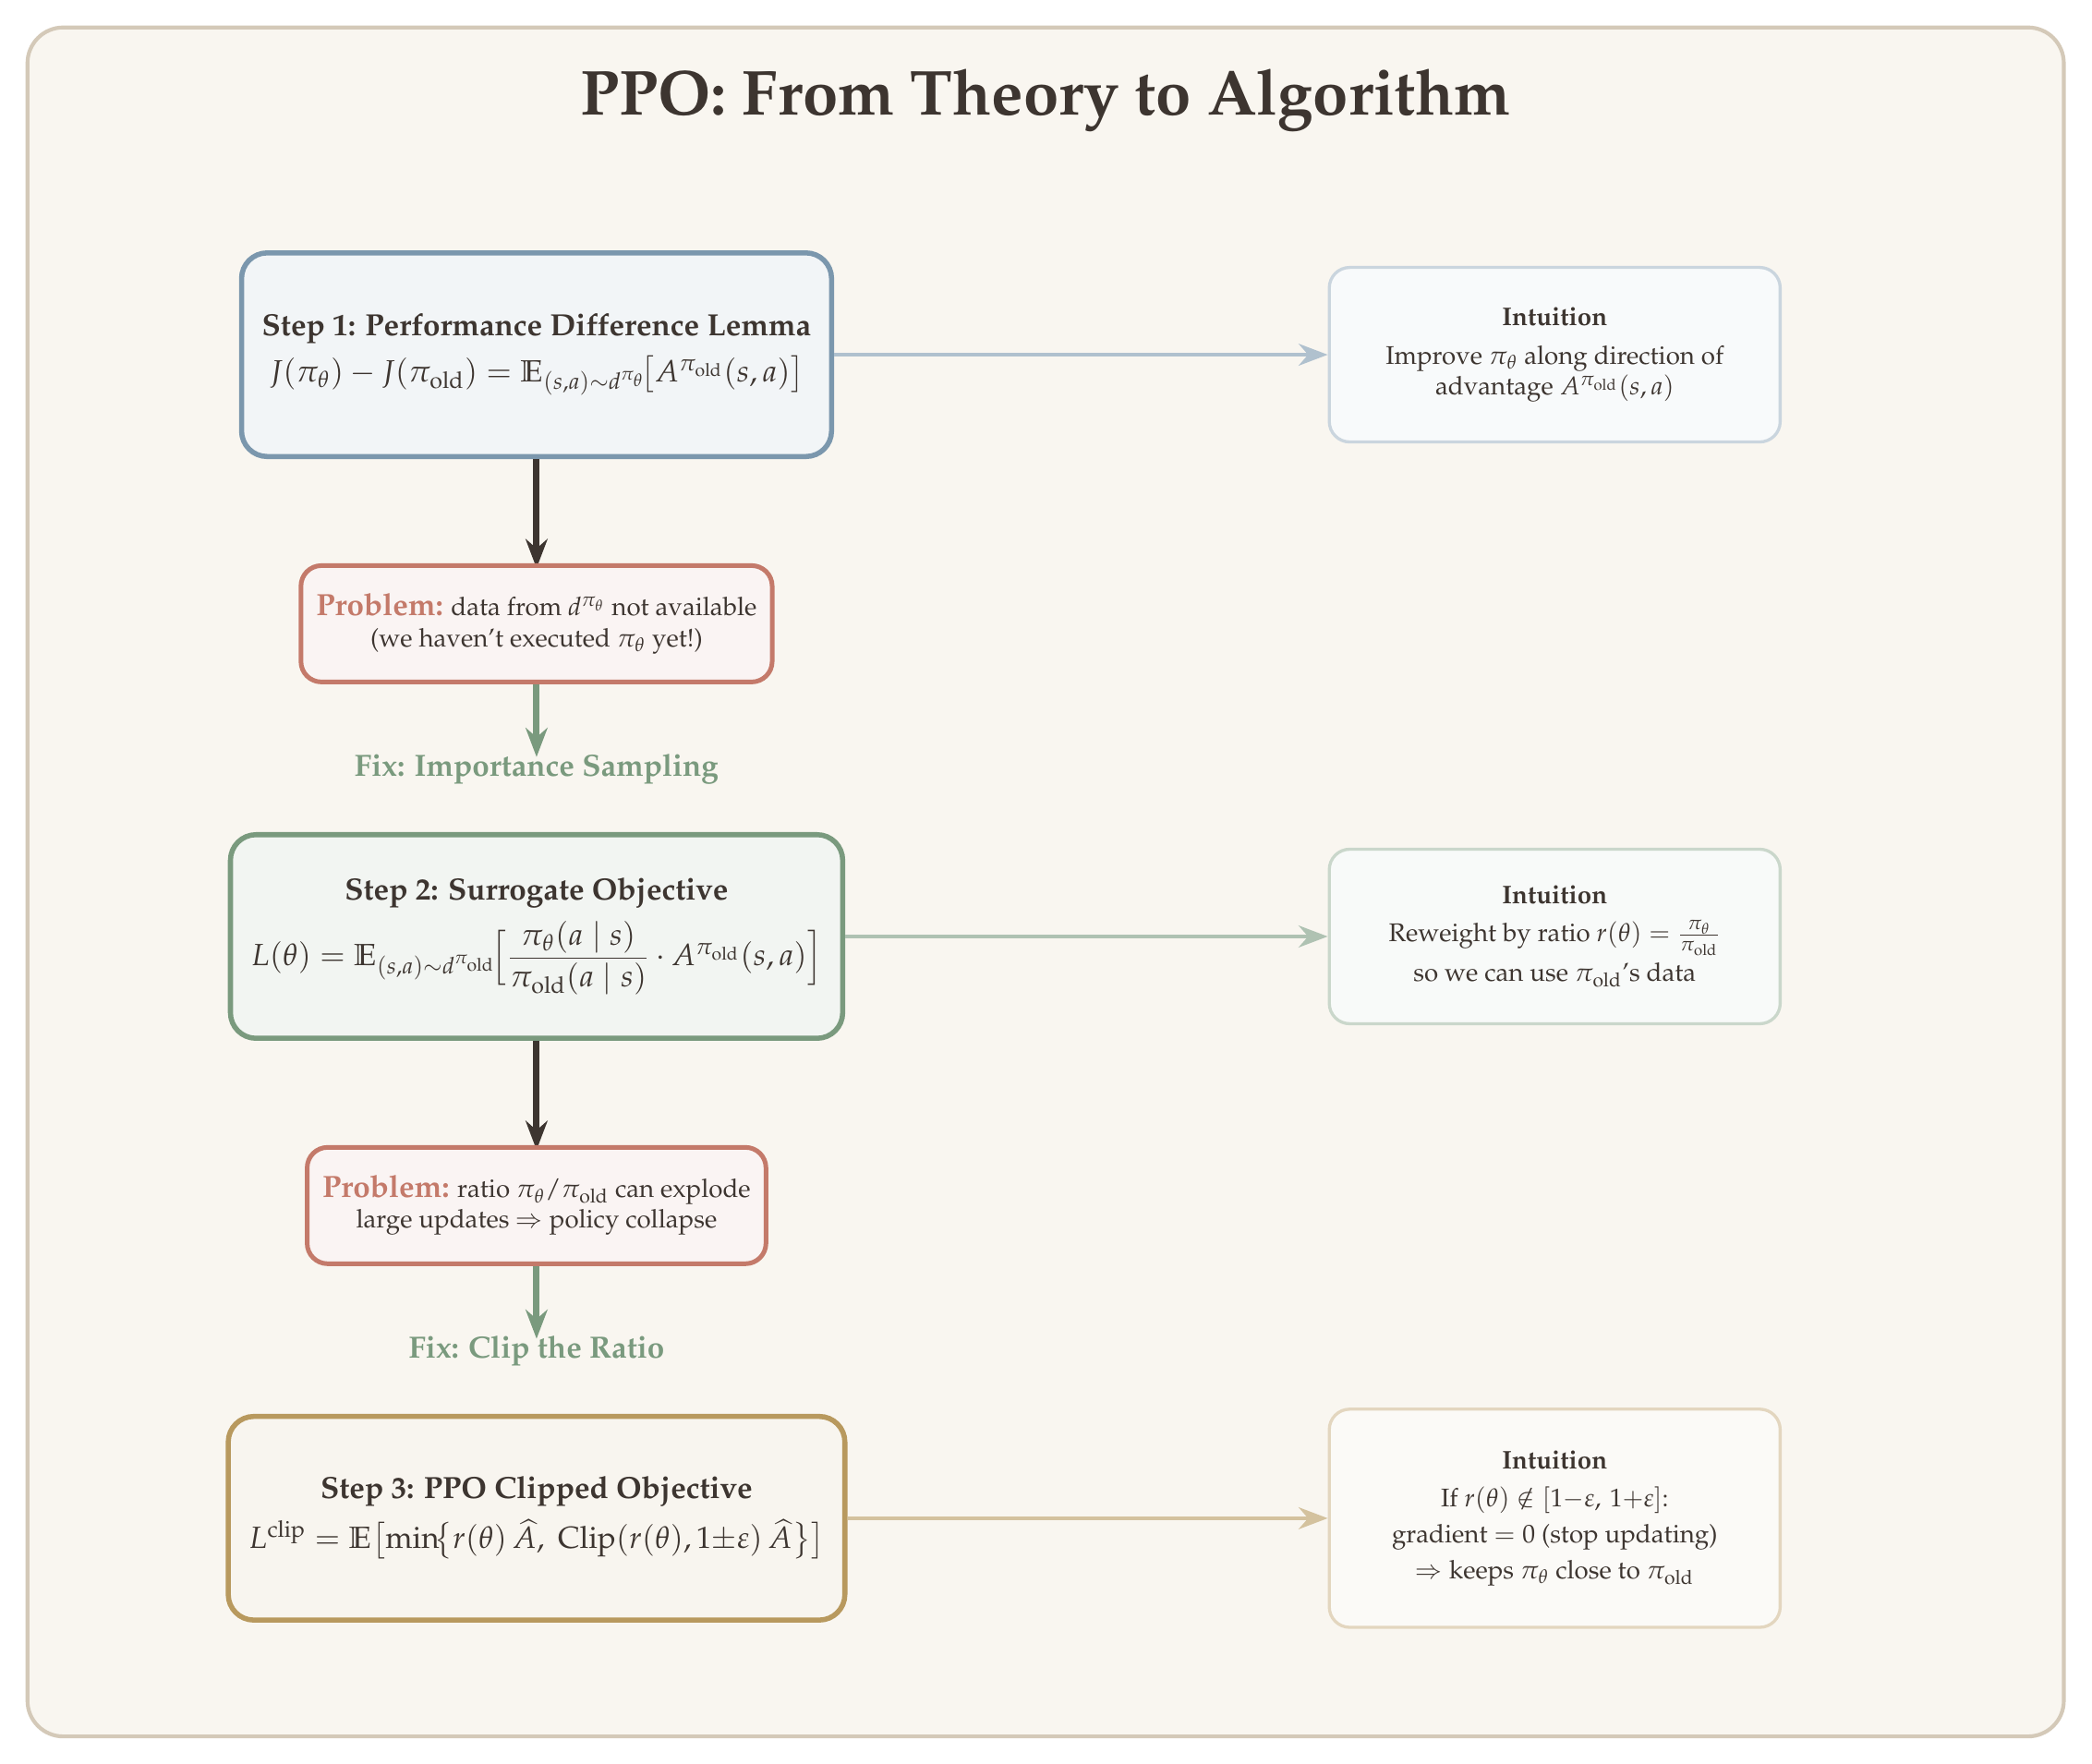
\begin{tikzpicture}[
  >={Stealth[length=4mm, width=3mm]},
  stepbox/.style={
    draw=#1, line width=2pt, fill=#1!10, rounded corners=10pt,
    minimum width=72mm, minimum height=28mm, font=\large, text=dkbrown,
    align=center, inner sep=8pt
  },
  issbox/.style={
    draw=terracotta, line width=1.8pt, fill=terracotta!8, rounded corners=8pt,
    minimum width=60mm, minimum height=16mm, font=\normalsize, text=dkbrown,
    align=center, inner sep=6pt
  },
  arr/.style={->, line width=2.5pt, dkbrown},
  problbl/.style={font=\large\bfseries, text=terracotta, align=center},
  fixlbl/.style={font=\large\bfseries, text=sage, align=center},
]

% Background
\fill[cream, rounded corners=14pt] (-2,-1.5) rectangle (26,22);
\draw[border, rounded corners=14pt, line width=1.5pt] (-2,-1.5) rectangle (26,22);

% Title
\node[font=\Huge\bfseries, text=dkbrown] at (12,21)
  {PPO: From Theory to Algorithm};

% =============================================
% Step 1: Performance Difference Lemma
% =============================================
\node[stepbox=stblue] (pdl) at (5,17.5)
  {\textbf{Step 1: Performance Difference Lemma}\\[4pt]
   $J(\pi_\theta) - J(\pi_{\text{old}})
   = \mathbb{E}_{(s,a) \sim d^{\pi_\theta}}\!\bigl[A^{\pi_{\text{old}}}(s,a)\bigr]$};

% Arrow down + problem
\draw[arr] (pdl.south) -- ++(0,-1.5);
\node[issbox] (prob1) at (5,13.8)
  {{\large\bfseries\color{terracotta} Problem:} data from $d^{\pi_\theta}$ not available\\
   {\normalsize (we haven't executed $\pi_\theta$ yet!)}};

% =============================================
% Step 2: Importance Sampling Fix
% =============================================
\draw[arr, sage] (prob1.south) -- ++(0,-1);
\node[font=\large\bfseries, text=sage] at (5,11.8) {Fix: Importance Sampling};

\node[stepbox=sage] (is) at (5,9.5)
  {\textbf{Step 2: Surrogate Objective}\\[4pt]
   $L(\theta) = \mathbb{E}_{(s,a) \sim d^{\pi_{\text{old}}}}
   \!\Bigl[\dfrac{\pi_\theta(a \mid s)}{\pi_{\text{old}}(a \mid s)} \cdot A^{\pi_{\text{old}}}(s,a)\Bigr]$};

% Arrow down + problem
\draw[arr] (is.south) -- ++(0,-1.5);
\node[issbox] (prob2) at (5,5.8)
  {{\large\bfseries\color{terracotta} Problem:} ratio $\pi_\theta/\pi_{\text{old}}$ can explode\\
   {\normalsize large updates $\Rightarrow$ policy collapse}};

% =============================================
% Step 3: Clipping
% =============================================
\draw[arr, sage] (prob2.south) -- ++(0,-1);
\node[font=\large\bfseries, text=sage] at (5,3.8) {Fix: Clip the Ratio};

\node[stepbox=rwgold] (clip) at (5,1.5)
  {\textbf{Step 3: PPO Clipped Objective}\\[4pt]
   $L^{\text{clip}} = \mathbb{E}\bigl[\min\!\bigl\{r(\theta)\,\widehat{A},\;
   \text{Clip}(r(\theta), 1{\pm}\varepsilon)\,\widehat{A}\bigr\}\bigr]$};

% =============================================
% Right side: Visual intuition for each step
% =============================================

% PDL intuition
\node[draw=stblue!40, line width=1.2pt, fill=stblue!5, rounded corners=8pt,
      minimum width=62mm, minimum height=24mm, font=\normalsize, text=dkbrown,
      align=center, inner sep=6pt]
  (pdl-int) at (19,17.5)
  {\textbf{Intuition}\\[3pt]
   Improve $\pi_\theta$ along direction of\\
   advantage $A^{\pi_{\text{old}}}(s,a)$};
\draw[->, line width=1.5pt, stblue!60] (pdl.east) -- (pdl-int.west);

% IS intuition
\node[draw=sage!40, line width=1.2pt, fill=sage!5, rounded corners=8pt,
      minimum width=62mm, minimum height=24mm, font=\normalsize, text=dkbrown,
      align=center, inner sep=6pt]
  (is-int) at (19,9.5)
  {\textbf{Intuition}\\[3pt]
   Reweight by ratio $r(\theta) = \frac{\pi_\theta}{\pi_{\text{old}}}$\\[2pt]
   so we can use $\pi_{\text{old}}$'s data};
\draw[->, line width=1.5pt, sage!60] (is.east) -- (is-int.west);

% Clip intuition
\node[draw=rwgold!40, line width=1.2pt, fill=rwgold!5, rounded corners=8pt,
      minimum width=62mm, minimum height=30mm, font=\normalsize, text=dkbrown,
      align=center, inner sep=6pt]
  (clip-int) at (19,1.5)
  {\textbf{Intuition}\\[3pt]
   If $r(\theta) \notin [1{-}\varepsilon,\, 1{+}\varepsilon]$:\\[2pt]
   gradient $= 0$ (stop updating)\\[2pt]
   $\Rightarrow$ keeps $\pi_\theta$ close to $\pi_{\text{old}}$};
\draw[->, line width=1.5pt, rwgold!60] (clip.east) -- (clip-int.west);

\end{tikzpicture}
\end{document}
